\chapter{Море Дирака, масса фермиона и четырёхкомпонентные спиноры}

\section{Праводвижущиеся фермионы и море Дирака}

Уравнение Дирака — это уравнение для фермионов. Релятивистские бозоны подчиняются другим уравнениям, таким как уравнение Клейна--Гордона или уравнения Максвелла. Простейший пример задаётся в одном пространственном измерении и сначала описывает частицы и античастицы, которые могут двигаться только вправо.

Начнём с плоской волны,
\begin{equation}
\psi(x,t)=\psi_0 e^{i(kx-\omega t)}.
\end{equation}
Её фазовая скорость равна
\begin{equation}
v_{\mathrm{ph}}=\frac{\omega}{k}.
\end{equation}
Знаки \(k\) и \(\omega\) существенны. Если они одного знака, фаза движется вправо; если разных знаков, она движется влево. Когда \(\omega\) пропорциональна \(k\), фазовая и групповая скорости совпадают:
\begin{equation}
v_{\mathrm{g}}=\frac{d\omega}{dk}=\frac{\omega}{k}.
\end{equation}

Рассмотрим уравнение первого порядка
\begin{equation}
\frac{\partial\psi}{\partial x}
+
\frac{\partial\psi}{\partial t}
=0.
\end{equation}
Подстановка плоской волны даёт
\begin{equation}
ik\psi-i\omega\psi=0,
\end{equation}
и, следовательно,
\begin{equation}
\omega=k.
\end{equation}
Поэтому волна движется вправо. Полезно обозначить поле соответственно:
\begin{equation}
\frac{\partial\psi_R}{\partial t}
=
-\frac{\partial\psi_R}{\partial x}.
\end{equation}

Восстанавливая скорость света, получаем размерную форму
\begin{equation}
\frac{\partial\psi_R}{\partial x}
+
\frac{1}{c}\frac{\partial\psi_R}{\partial t}
=0,
\end{equation}
так что
\begin{equation}
\omega=ck.
\end{equation}
Отныне \(c=1\). При \(\hbar=1\) величина \(\omega\) также является энергией одного кванта.

\begin{figure}[htbp]
\centering
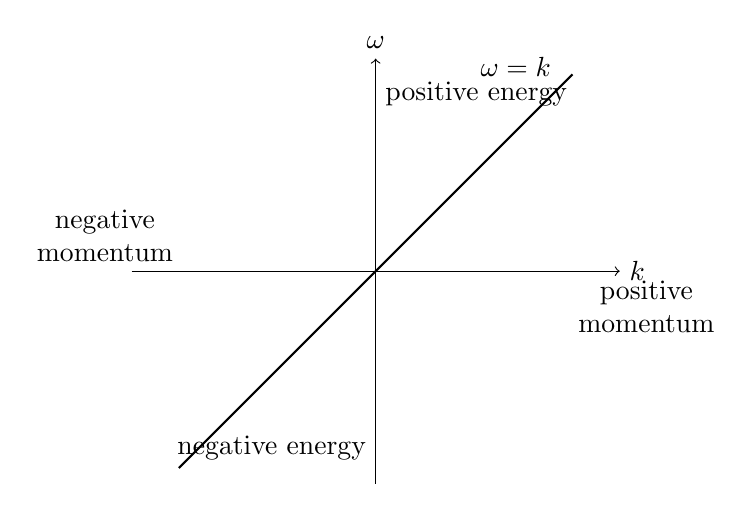
\begin{tikzpicture}[scale=1.0]
\draw[->] (-3.1,0) -- (3.1,0) node[right] {$k$};
\draw[->] (0,-2.7) -- (0,2.7) node[above] {$\omega$};
\draw[thick] (-2.5,-2.5) -- (2.5,2.5);
\node[above left] at (2.35,2.35) {$\omega=k$};
\node[below right,align=center] at (2.45,0) {positive\\momentum};
\node[above left,align=center] at (-2.45,0) {negative\\momentum};
\node[right] at (0,2.25) {positive energy};
\node[left] at (0,-2.25) {negative energy};
\end{tikzpicture}
\caption{Безмассовое праводвижущееся соотношение дисперсии \(\omega=k\) содержит ветви положительной и отрицательной энергии.}
\end{figure}

Из этой прямой вытекает серьёзное следствие. Положительное \(k\) даёт положительную энергию, тогда как отрицательное \(k\) даёт отрицательную энергию. Тем не менее обе части описывают волны, движущиеся вправо, поскольку \(\omega/k=1\) на всей прямой.

Электрон, помещённый на ветвь с положительной энергией, мог бы перейти в состояние с меньшей энергией, испустить фотон с положительной энергией, снова перейти ниже и продолжать спускаться по спектру: на одну ступень, потом на другую и ещё на одну. Ни один электрон не был бы устойчив. Более серьёзно, мир понижал бы свою энергию, рождая всё больше и больше электронов с отрицательной энергией.

Принцип запрета для фермионов даёт выход. Заполним каждое электронное состояние с отрицательной энергией. Второй электрон не может попасть в уже занятое состояние, поэтому полностью заполненный сектор отрицательных энергий препятствует неограниченному падению. Этот заполненный сектор — море Дирака, а его полностью заполненное состояние есть основное состояние, или вакуум.

\begin{classroomqa}
\lecturetimestamp{00:07:19}
\audiencequestion{Существует ли бесконечно много более низких состояний с отрицательной энергией?}
\lecturerresponse{Да. При дискретных импульсах спектр похож на бесконечную лестницу; при непрерывных импульсах — на непрерывную горку. Заполнение моря отрицательной энергии не даёт электрону опускаться бесконечно, хотя конечный переход вниз с испусканием фотона всё ещё может быть возможен, если доступно незанятое более низкое состояние.}
\end{classroomqa}

Это объясняет, почему уравнение с таким спектром должно квантоваться как фермионная теория. Если бы кванты были бозонами, сколь угодно многие из них могли бы занимать одно и то же более низкое состояние, и заполнение сектора отрицательных энергий не стабилизировало бы вакуум.

Картина заполненного моря также порождает античастицы. В вакууме все уровни с отрицательной энергией заняты, а все уровни с положительной энергией пусты. Электрон можно перевести с любого занятого уровня отрицательной энергии на любой незанятый уровень положительной энергии; начальный и конечный уровни не обязаны располагаться симметрично.

\begin{figure}[htbp]
\centering
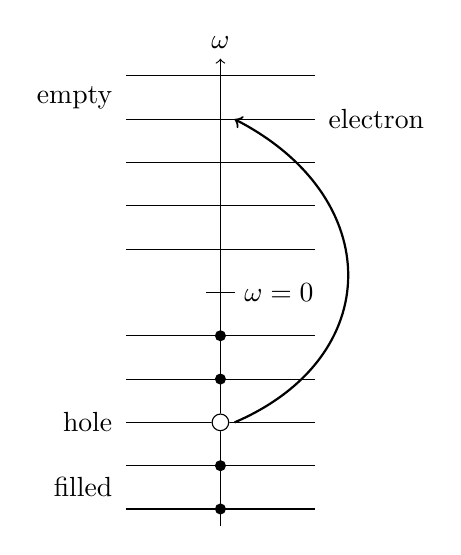
\begin{tikzpicture}[x=1cm,y=0.55cm]
\draw[->] (0,-5.4) -- (0,5.4) node[above] {$\omega$};
\draw (-0.18,0) -- (0.18,0) node[right] {$\omega=0$};
\foreach \y in {-5,-4,-3,-2,-1} {
  \draw (-1.2,\y) -- (1.2,\y);
  \fill (0,\y) circle (2pt);
}
\foreach \y in {1,2,3,4,5} {
  \draw (-1.2,\y) -- (1.2,\y);
}
\draw[->,thick] (0.18,-3) .. controls (2.1,-1.5) and (2.1,2.2) .. (0.18,4);
\draw[white,fill=white] (0,-3) circle (3pt);
\draw (0,-3) circle (3pt);
\node[left] at (-1.25,-3) {hole};
\node[left] at (-1.25,-4.5) {filled};
\node[left] at (-1.25,4.5) {empty};
\node[right] at (1.25,4) {electron};
\end{tikzpicture}
\caption{Перевод занятого электрона с отрицательной энергией создаёт электрон с положительной энергией и оставляет дырку в заполненном море.}
\end{figure}

Удаление электрона с отрицательной энергией повышает энергию относительно вакуума, поэтому дырка имеет положительную энергию. На ветви \(\omega=k\) удалённый электрон имел также отрицательный импульс. Удаление отрицательного импульса оставляет положительный избыток импульса, поэтому дырка имеет положительный импульс. Если заряд электрона считать отрицательным, то у отсутствующего электрона заряд положителен. Таким образом, дырка — это античастица с положительной энергией и положительным импульсом, тогда как переведённый электрон имеет отрицательный заряд, положительную энергию и положительный импульс. В этой теории с одной ветвью всякое реальное возбуждение движется вправо.

Поле \(\psi_R\) строится из фермионных операторов рождения и уничтожения. Поэтому интерпретация через частицы и дырки есть утверждение о квантах, создаваемых и уничтожаемых полем, а не только о классической волне.

Однако асимметрия всё ещё остаётся. Праводвижущееся море содержит состояния с отрицательной энергией и отрицательным импульсом. Его формальный полный импульс огромен и направлен влево. Можно определить импульс вакуума равным нулю, вычитая эту константу, но состояние остаётся структурно несбалансированным: частицы и античастицы движутся только вправо, тогда как заполненный вакуум составлен из состояний с отрицательным импульсом.

\section{Леводвижущаяся ветвь и сбалансированный вакуум}

Баланс между левым и правым направлениями требует второго, независимого поля со своими собственными операторами рождения и уничтожения. Пусть оно удовлетворяет
\begin{equation}
\frac{\partial\psi_L}{\partial t}
=
+\frac{\partial\psi_L}{\partial x}.
\end{equation}
Для той же формы плоской волны
\begin{equation}
-i\omega\psi_L=ik\psi_L,
\end{equation}
так что
\begin{equation}
\omega=-k.
\end{equation}
Эта вторая прямая является зеркальным отражением \(\omega=k\). Её ветвь с положительной энергией описывает частицы, движущиеся влево, и её ветвь с отрицательной энергией тоже должна быть заполнена.

\begin{figure}[htbp]
\centering
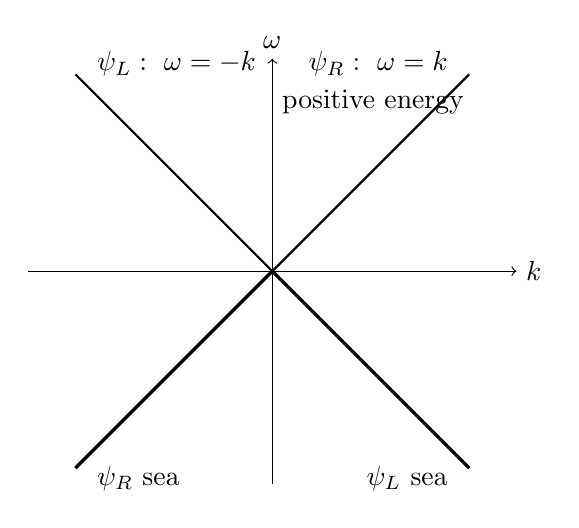
\begin{tikzpicture}[scale=1.0]
\draw[->] (-3.1,0) -- (3.1,0) node[right] {$k$};
\draw[->] (0,-2.7) -- (0,2.7) node[above] {$\omega$};
\draw[thick] (-2.5,-2.5) -- (2.5,2.5);
\draw[thick] (-2.5,2.5) -- (2.5,-2.5);
\draw[very thick] (-2.5,-2.5) -- (0,0);
\draw[very thick] (0,0) -- (2.5,-2.5);
\node[above left] at (2.35,2.35) {$\psi_R:\ \omega=k$};
\node[above right] at (-2.35,2.35) {$\psi_L:\ \omega=-k$};
\node[right] at (0,2.15) {positive energy};
\node[below right] at (-2.35,-2.35) {$\psi_R$ sea};
\node[below left] at (2.35,-2.35) {$\psi_L$ sea};
\end{tikzpicture}
\caption{Независимые поля, движущиеся вправо и влево, дают зеркальные безмассовые ветви; в вакууме заполнены две полуветви отрицательной энергии.}
\end{figure}

После заполнения обоих морей отрицательной энергии число занятых леводвижущихся состояний становится таким же, как и праводвижущихся. Их вакуумные импульсы уравновешиваются. Теперь частичные и дырочные возбуждения могут двигаться в любом направлении.

\begin{classroomqa}
\lecturetimestamp{00:15:58}
\audiencequestion{Можно ли решить проблему отрицательной энергии, не постулируя заполненные состояния и дырки?}
\lecturerresponse{Ту же самую теорию можно переобозначить. Заполненное электронное состояние с отрицательной энергией можно назвать пустым состоянием античастицы; тогда в физическом языке останутся только частицы и античастицы с положительной энергией. Картина заполненного моря остаётся полезной проверкой на согласованность, подобно заполненной зоне в металле, где удаление электрона создаёт дырку, а перевод на более высокий уровень создаёт и частицу, и дырку.}
\end{classroomqa}

Рассмотренные до сих пор возбуждения безмассовы. Их дисперсионные соотношения линейны, а модули их скоростей равны \(1\), так что они движутся со скоростью света. Следующий вопрос состоит в том, как наделить их массой.

\section{Две компоненты и массовый член}

Сначала объединим два поля в столбец:
\begin{equation}
\Psi=
\begin{pmatrix}
\psi_R\\
\psi_L
\end{pmatrix}.
\end{equation}
Изначально это лишь компактная запись двух независимых уравнений. Определим
\begin{equation}
\alpha=
\begin{pmatrix}
1&0\\
0&-1
\end{pmatrix}.
\end{equation}
Тогда уравнения для праводвижущегося и леводвижущегося полей принимают вид
\begin{equation}
\frac{\partial\Psi}{\partial t}
=
-\alpha\frac{\partial\Psi}{\partial x}.
\end{equation}

\begin{figure}[htbp]
\centering
\includegraphics[width=0.78\textwidth]{lecture_06_figure_02.png}
\caption{Поля \(\psi_R\) и \(\psi_L\) образуют двухкомпонентный спинор, причём \(\alpha\) различает две безмассовые ветви.}
\lectureframe{00:20:36}
\end{figure}

Для плоской волны операторы
\begin{equation}
i\partial_t
\quad\hbox{and}\quad
-i\partial_x
\end{equation}
дают соответственно \(\omega\) и \(k\). Поэтому матричное уравнение можно сокращённо записать как
\begin{equation}
\omega=\alpha k.
\end{equation}
Для верхней компоненты это означает \(\omega=k\); для нижней — \(\omega=-k\). Эта запись сжала два уравнения, но не внесла никакой новой физики.

Электроны не безмассовы и не движутся со скоростью света. Заманчивой формулой для их энергии является нерелятивистская кинетическая энергия \(k^2/(2m)\), но здесь она не может служить отправной точкой: безмассовый предел уже относится к движению со скоростью света. Релятивистское соотношение имеет вид
\begin{equation}
\omega^2=k^2+m^2,
\end{equation}
или, если включить обе энергетические ветви,
\begin{equation}
\omega=\pm\sqrt{k^2+m^2}.
\end{equation}
При \(m=0\) они переходят в \(\omega=k\) и \(\omega=-k\).

\begin{classroomqa}
\lecturetimestamp{00:25:23}
\audiencequestion{Используются ли единицы с \(c=1\), и как получается скорость массивной частицы?}
\lecturerresponse{Да. Скорость волнового пакета — это групповая скорость, \(v_{\mathrm g}=d\omega/dk=k/\sqrt{k^2+m^2}\) на ветви с положительной энергией. Таким образом, само дисперсионное соотношение уже содержит уменьшение скорости ниже \(c=1\) для массивной частицы.}
\end{classroomqa}

\begin{classroomqa}
\lecturetimestamp{00:26:29}
\audiencequestion{Является ли \(\omega\) в сокращении \(\omega=\alpha k\) вектором или матрицей?}
\lecturerresponse{Эта сокращённая запись обозначает операторное уравнение, действующее на двухкомпонентную волновую функцию. Здесь \(\omega\) означает \(i\partial_t\), \(k\) означает \(-i\partial_x\), а \(\alpha\) — это матрица, действующая на индекс компоненты. Скалярные символы \(\omega\) и \(k\) становятся своими численными собственными значениями только для плоской волны.}
\end{classroomqa}

Сохраним уравнение первого порядка и попробуем простейшее зависящее от массы обобщение:
\begin{equation}
\omega=\alpha k+\beta m.
\end{equation}
Объект \(\beta\) должен быть матрицей, потому что он действует на то же двухкомпонентное поле, что и \(\alpha\). Его алгебра следует из возведения в квадрат:
\begin{align}
\omega^2
&=(\alpha k+\beta m)(\alpha k+\beta m)\\
&=\alpha^2k^2+\beta^2m^2
+\alpha\beta\,km+\beta\alpha\,mk\\
&=\alpha^2k^2+\beta^2m^2
+(\alpha\beta+\beta\alpha)km.
\end{align}
Чтобы получить \(k^2+m^2\) при любых \(k\) и \(m\), требуется
\begin{equation}
\alpha^2=I,
\qquad
\beta^2=I,
\qquad
\alpha\beta+\beta\alpha=0.
\end{equation}

Два обычных ненулевых числа не могут удовлетворить последнему условию: для чисел из него следовало бы \(2\alpha\beta=0\), что противоречит тому, что оба квадрата равны \(1\). Матрицы могут антикоммутировать. В частности, \(\beta\) не может совпадать с \(\alpha\), поскольку тогда
\begin{equation}
\alpha\beta+\beta\alpha=2\alpha^2=2I.
\end{equation}

Выберем
\begin{equation}
\beta=
\begin{pmatrix}
0&1\\
1&0
\end{pmatrix}.
\end{equation}
Ее квадрат можно проверить поэлементно:
\begin{equation}
\begin{aligned}
\beta^2
&=
\begin{pmatrix}
0&1\\
1&0
\end{pmatrix}
\begin{pmatrix}
0&1\\
1&0
\end{pmatrix}\\
&=
\begin{pmatrix}
0\cdot0+1\cdot1&0\cdot1+1\cdot0\\
1\cdot0+0\cdot1&1\cdot1+0\cdot0
\end{pmatrix}
=
\begin{pmatrix}
1&0\\
0&1
\end{pmatrix}.
\end{aligned}
\end{equation}
Порядок умножения существен:
\begin{align}
\alpha\beta
&=
\begin{pmatrix}
1&0\\
0&-1
\end{pmatrix}
\begin{pmatrix}
0&1\\
1&0
\end{pmatrix}
=
\begin{pmatrix}
0&1\\
-1&0
\end{pmatrix},\\
\beta\alpha
&=
\begin{pmatrix}
0&1\\
1&0
\end{pmatrix}
\begin{pmatrix}
1&0\\
0&-1
\end{pmatrix}
=
\begin{pmatrix}
0&-1\\
1&0
\end{pmatrix}.
\end{align}
Следовательно,
\begin{equation}
\alpha\beta=-\beta\alpha,
\qquad
\alpha\beta+\beta\alpha=0.
\end{equation}
Возможны и другие эквивалентные выборы матрицы, но этот делает уравнения для компонент особенно наглядными.

Восстанавливая дифференциальные операторы, получаем уравнение с массовым членом
\begin{equation}
i\frac{\partial\Psi}{\partial t}
=
-i\alpha\frac{\partial\Psi}{\partial x}
+m\beta\Psi.
\end{equation}
Матрица \(\beta\) меняет две компоненты местами:
\begin{equation}
\beta
\begin{pmatrix}
\psi_R\\
\psi_L
\end{pmatrix}
=
\begin{pmatrix}
\psi_L\\
\psi_R
\end{pmatrix}.
\end{equation}
Следовательно,
\begin{align}
i\dot{\psi}_R
&=-i\frac{\partial\psi_R}{\partial x}+m\psi_L,\\
i\dot{\psi}_L
&=+i\frac{\partial\psi_L}{\partial x}+m\psi_R.
\end{align}

Массовый член связывает поля, которые в безмассовой теории были независимыми. Уравнение для верхней компоненты содержит нижнюю компоненту, а уравнение для нижней компоненты — верхнюю. Именно такое связывание и означает масса Дирака. Уравнения инвариантны относительно трансляций, поэтому импульс сохраняется, а масса соответствующих частиц равна \(m\).

\begin{classroomqa}
\lecturetimestamp{00:38:25}
\audiencequestion{Является ли решение автоматически лоренц-инвариантным?}
\lecturerresponse{Отдельное решение не должно оставаться неизменным при преобразовании Лоренца. Состояние с определенным импульсом переходит в состояние с преобразованным импульсом, так что правильное утверждение здесь — ковариантность. Соотношение \(\omega^2=k^2+m^2\) — одна из ключевых лоренц-инвариантных проверок, но полная ковариантность требует также закона преобразования спинора \(\Psi\), который пока еще не установлен.}
\end{classroomqa}

\section{Система покоя и смысл компонент}

Безмассовую частицу нельзя привести в состояние покоя, а массивную можно. В системе покоя \(k=0\), поэтому волновая функция не зависит от координаты, и
\begin{equation}
\omega=\beta m.
\end{equation}
Дифференциальное уравнение сводится к виду
\begin{equation}
i\frac{d\Psi}{dt}=m\beta\Psi.
\end{equation}
В компонентах
\begin{align}
i\dot{\psi}_R&=m\psi_L,\\
i\dot{\psi}_L&=m\psi_R.
\end{align}
Оба внедиагональных элемента \(\beta\) равны \(+1\), так что ни в одном из этих уравнений не появляется дополнительный минус.

Уравнения расцепляются после сложения и вычитания компонент. Введем
\begin{equation}
\psi_+=\psi_R+\psi_L,
\qquad
\psi_-=\psi_R-\psi_L.
\end{equation}
Сложение двух уравнений в системе покоя дает
\begin{equation}
i\dot{\psi}_+=m\psi_+,
\end{equation}
а вычитание дает
\begin{equation}
i\dot{\psi}_-=-m\psi_-.
\end{equation}
Следовательно,
\begin{equation}
\omega=+m
\quad\hbox{for }\psi_+,
\qquad
\omega=-m
\quad\hbox{for }\psi_-.
\end{equation}

\begin{figure}[htbp]
\centering
\includegraphics[width=0.62\textwidth]{lecture_06_figure_03.png}
\caption{При нулевом импульсе \(\psi_+=\psi_R+\psi_L\) и \(\psi_-=\psi_R-\psi_L\) имеют частоты покоя \(\omega=+m\) и \(\omega=-m\).}
\lectureframe{00:44:49}
\end{figure}

Положительноэнергетическое поле в системе покоя — \(\psi_+\); отрицательноэнергетическое — \(\psi_-\). Состояния с отрицательной энергией заполнены, как и прежде. Результат в системе покоя — лишь срез полного спектра при \(k=0\):
\begin{equation}
\omega_\pm(k)=\pm\sqrt{k^2+m^2}.
\end{equation}
\begin{figure}[htbp]
\centering
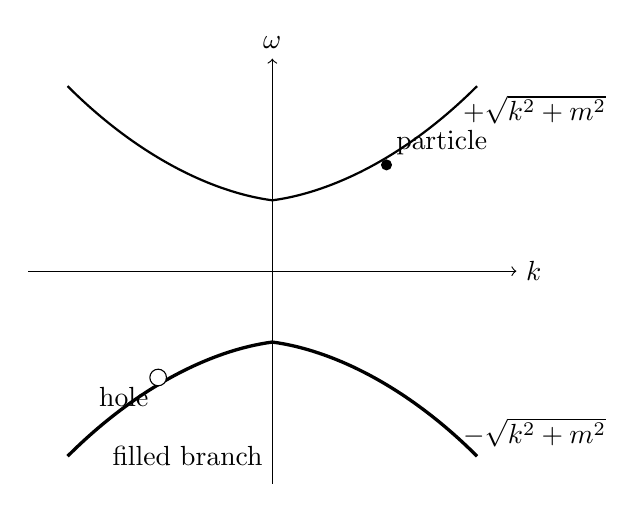
\begin{tikzpicture}[scale=1.0]
\draw[->] (-3.1,0) -- (3.1,0) node[right] {$k$};
\draw[->] (0,-2.7) -- (0,2.7) node[above] {$\omega$};
\draw[thick] (-2.6,2.35)
  .. controls (-1.7,1.45) and (-0.75,1.0) .. (0,0.9)
  .. controls (0.75,1.0) and (1.7,1.45) .. (2.6,2.35);
\draw[very thick] (-2.6,-2.35)
  .. controls (-1.7,-1.45) and (-0.75,-1.0) .. (0,-0.9)
  .. controls (0.75,-1.0) and (1.7,-1.45) .. (2.6,-2.35);
\fill (1.45,1.35) circle (2pt);
\node[above right] at (1.45,1.35) {particle};
\fill[white] (-1.45,-1.35) circle (3pt);
\draw (-1.45,-1.35) circle (3pt);
\node[below left] at (-1.45,-1.35) {hole};
\node[right] at (2.3,2.05) {$+\sqrt{k^2+m^2}$};
\node[right] at (2.3,-2.05) {$-\sqrt{k^2+m^2}$};
\node[left] at (0,-2.35) {filled branch};
\end{tikzpicture}
\caption{При любом импульсе массивный спектр содержит состояния с положительной и отрицательной энергией. Отрицательная ветвь заполнена, и отсутствующее в ней состояние представляет собой дырку с положительной энергией.}
\end{figure}
Для каждого импульса есть состояние с положительной и состояние с отрицательной энергией. Если заполнить все состояния на отрицательной ветви, то над морем остаются частицы с положительной энергией, а в нем — дырки с положительной энергией. И частицы, и дырки имеют положительную массу.

Существенный момент заслуживает повторения. Фермион становится массивным, когда связываются две его прежде независимые компоненты. В системе покоя ни одна из исходных компонент по отдельности не является собственным состоянием энергии. Состояния с определенной энергией — это их сумма и разность.

Чтобы понять, что означает сумма, обозначим соответствующие одночастичные операторы рождения через \(C_R^\dagger\) и \(C_L^\dagger\). При действии на вакуум выражение
\begin{equation}
(C_R^\dagger+C_L^\dagger)\lvert0\rangle
\end{equation}
создает одну частицу в когерентной суперпозиции двух компонент. Оно не создает две частицы. А произведение,
\begin{equation}
C_R^\dagger C_L^\dagger\lvert0\rangle,
\end{equation}
содержит два оператора рождения и создает двухчастичное состояние, когда доступны обе моды. После нормировки состояние покоя дает равные вероятности для двух компонент, но связанная волна в целом имеет нулевой импульс.

Обозначения \(R\) и \(L\) буквально обозначали направление движения только при \(m=0\). Как только появляется массовый член, движущееся массивное решение, как правило, содержит обе компоненты, а решение в системе покоя содержит их с одинаковыми модулями. Поэтому здесь лучше рассматривать \(R\) и \(L\) как обозначения верхней и нижней компонент спинора.

\begin{figure}[htbp]
\centering
\includegraphics[width=0.78\textwidth]{lecture_06_figure_04.png}
\caption{При ненулевой массе две компоненты спинора связаны; интерпретация этих двух компонент как движущихся вправо и влево непосредственно применима только в безмассовом пределе.}
\lectureframe{00:50:48}
\end{figure}

Все массивные фермионы в физике элементарных частиц строятся из полей левой и правой компонент: масса Дирака связывает компоненты, которые в безмассовом пределе независимы.

\begin{classroomqa}
\lecturetimestamp{00:52:01}
\audiencequestion{Должно ли \(\psi_R\pm\psi_L\) включать множитель \(1/\sqrt{2}\)?}
\lecturerresponse{Его можно включить для нормировки состояния. Он умножает обе части уравнения и потому не изменяет уравнение движения.}
\end{classroomqa}

\begin{classroomqa}
\lecturetimestamp{00:52:12}
\audiencequestion{Имеют ли значение относительные величины правой и левой компонент?}
\lecturerresponse{Для выбранных собственных состояний в системе покоя их модули равны. Общая нормировка произвольна, но относительные величины фиксируются собственным вектором \(\beta\).}
\end{classroomqa}

\begin{classroomqa}
\lecturetimestamp{00:52:52}
\audiencequestion{Могут ли две компоненты иметь относительную фазу?}
\lecturerresponse{Да. Вещественные коэффициенты в \(\psi_R\pm\psi_L\) следуют из выбора вещественной \(\beta\). Другие матрицы, квадрат которых равен единице и которые антикоммутируют с \(\alpha\), являются эквивалентными выборами, и тогда между компонентами может появиться относительная фаза. После выбора представления его нужно использовать последовательно.}
\end{classroomqa}

\begin{classroomqa}
\lecturetimestamp{00:53:43}
\audiencequestion{Являются ли метки ``леводвижущийся'' и ``праводвижущийся'' вводящими в заблуждение после введения массы?}
\lecturerresponse{Отчасти. В безмассовой теории они описывают подлинные волны, движущиеся влево и вправо. При ненулевой массе даже частица, движущаяся в одном направлении, как правило, содержит обе компоненты, так что ``верхняя компонента'' и ``нижняя компонента'' — более безопасные обозначения.}
\end{classroomqa}

\begin{classroomqa}
\lecturetimestamp{00:55:01}
\audiencequestion{Требует ли фермион в покое уже спинового углового момента?}
\lecturerresponse{Нет, не в этой одномерной модели. В одном пространственном измерении угловой момент не определен, поэтому спин пока еще не вошел в построение.}
\end{classroomqa}

\begin{classroomqa}
\lecturetimestamp{00:55:24}
\audiencequestion{Содержит ли волновая функция фермионные операторы рождения и уничтожения?}
\lecturerresponse{Да.}
\end{classroomqa}

\begin{classroomqa}
\lecturetimestamp{00:55:30}
\audiencequestion{Где, помимо выбора операторов рождения и уничтожения, проявляется фермионный характер?}
\lecturerresponse{Он входит через фермионные правила рождения--уничтожения. Уравнение с таким спектром отрицательных энергий должно квантоваться по этим правилам; бозонные правила заполнения оставили бы вакуум неустойчивым. Релятивистские бозоны должны описываться другим волновым уравнением.}
\end{classroomqa}

\begin{classroomqa}
\lecturetimestamp{00:56:20}
\audiencequestion{Можно ли лоренцевым преобразованием перевести решение с ненулевым импульсом в решение в системе покоя?}
\lecturerresponse{Да. Буст может перевести массивное решение в его систему покоя, но для явного выполнения этого преобразования нужно знать, как преобразования Лоренца действуют на спинор \(\Psi\).}
\end{classroomqa}

\section{Масса из скалярного вакуумного поля}

\begin{classroomqa}
\lecturetimestamp{00:58:11}
\audiencequestion{Как взаимодействие с полем Хиггса порождает массовый член Дирака?}
\lecturerresponse{Замените постоянный коэффициент массы связью со скалярным полем. Если это поле обращается в нуль в вакууме, фермион остается безмассовым; если же оно имеет постоянное ненулевое вакуумное значение, связь действует в точности как масса.}
\end{classroomqa}

Пусть \(\phi(x,t)\) — скалярное поле со своим собственным уравнением движения. В уравнении Дирака заменим постоянный коэффициент \(m\) в массовом члене на \(g\phi(x,t)\):\footnote{Показанный член взаимодействия получается этой заменой в ранее установленном массовом члене \(m\beta\Psi\).}
\begin{equation}
i\frac{\partial\Psi}{\partial t}
=
-i\alpha\frac{\partial\Psi}{\partial x}
+g\phi(x,t)\,\beta\Psi.
\end{equation}
Тогда два уравнения поля оказываются связанными. Фермион действует на скалярное поле, а скалярное поле действует обратно на фермион; если рассматривать их вместе, система нелинейна, хотя уравнение Дирака линейно по \(\Psi\) при заданном \(\phi\).

Предположим сначала, что в пустом пространстве
\begin{equation}
\phi(x,t)=0.
\end{equation}
Тогда член смешивания обращается в нуль, верхняя и нижняя компоненты расцепляются, и фермион безмассов. Предположим вместо этого, что состояние наименьшей энергии имеет постоянное ненулевое скалярное поле,
\begin{equation}
\phi(x,t)=\phi_0\neq0.
\end{equation}
Тогда уравнение Дирака в таком вакууме принимает вид
\begin{equation}
i\frac{\partial\Psi}{\partial t}
=
-i\alpha\frac{\partial\Psi}{\partial x}
+g\phi_0\,\beta\Psi,
\end{equation}
так что
\begin{equation}
m_{\mathrm{eff}}=g\phi_0.
\end{equation}
Следовательно, связь между бозонным полем и фермионным полем вместе с ненулевым значением бозонного поля в пустом пространстве порождает то же смешивание левой и правой компонент, которое раньше возникало как масса, прямо вписанная в уравнение.

\begin{classroomqa}
\lecturetimestamp{01:01:27}
\audiencequestion{Может ли LHC дать свидетельства того, что поле Хиггса в вакууме ненулевое?}
\lecturerresponse{Безусловно. Это один из главных вопросов.}
\end{classroomqa}

\begin{classroomqa}
\lecturetimestamp{01:01:32}
\audiencequestion{Не могли бы вы подробнее объяснить, как работает механизм Хиггса?}
\lecturerresponse{Со скалярным полем связана энергия, обусловленная его изменением в пространстве и времени, и оно также может обладать локальной потенциальной энергией \(V(\phi)\). Если минимумы этого потенциала достигаются при ненулевых значениях \(\phi\), вакуум содержит ненулевое поле. Квантованные колебания около выбранного минимума — это частицы Хиггса.}
\end{classroomqa}

Поле может нести энергию двумя различными способами. Часть энергии зависит от того, как поле меняется в пространстве и времени. Поле Максвелла — привычный пример для сравнения:
\begin{equation}
\mathcal{E}_{\mathrm{Maxwell}}\propto \mathbf E^2+\mathbf B^2,
\end{equation}
и и \(\mathbf E\), и \(\mathbf B\) выражаются через производные электромагнитного потенциала. Следовательно, эта энергия связана с пространственно-временным изменением лежащего в основе поля.

Скалярное поле может также иметь локальную плотность потенциальной энергии,
\begin{equation}
V(\phi),
\end{equation}
которая зависит от значения самого \(\phi\), а не от его производных. Схематически,
\begin{equation}
\mathcal{E}_\phi
=
\mathcal E_{\text{space and time gradients}}+V(\phi).
\end{equation}
При отсутствии более глубокого принципа, который её фиксировал бы, \(V(\phi)\) могла бы быть любой разумной функцией, совместимой с симметриями модели.

Для упрощённой иллюстрации с вещественным скалярным полем, используемой здесь, будем считать, что теория симметрична относительно преобразования
\begin{equation}
\phi\longrightarrow-\phi.
\end{equation}
Тогда потенциал должен быть чётной функцией:
\begin{equation}
V(\phi)=V(-\phi).
\end{equation}
Одна лишь эта симметрия не говорит, где расположен минимум. Один вариант — единственный минимум при \(\phi=0\). Другой — симметричная пара минимумов при ненулевых значениях, один положительный и один отрицательный.

\begin{figure}[htbp]
\centering
\includegraphics[width=0.72\textwidth]{lecture_06_figure_05.png}
\caption{Минимум при \(\phi=0\) даёт нулевое вакуумное поле, тогда как симметричные ненулевые минимумы допускают вакуумное значение \(\phi_0\neq0\) и, следовательно, массу фермиона \(g\phi_0\).}
\lectureframe{01:04:47}
\end{figure}

Эти две возможности можно изобразить, не задаваясь конкретной полиномиальной формой потенциала.\footnote{На приведённых ниже кривых сохранены лишь качественные особенности — центральный минимум и симметрично связанные минимумы, — используемые в рассуждении.}
\begin{figure}[htbp]
\centering
\resizebox{\linewidth}{!}{%
\begin{tikzpicture}[x=1.35cm,y=1.05cm]
\begin{scope}[shift={(-3.1,0)}]
\draw[->] (-1.7,0) -- (1.7,0) node[right] {$\phi$};
\draw[->] (0,-0.15) -- (0,2.45) node[above] {$V(\phi)$};
\draw[thick] (-1.5,2.05) .. controls (-0.9,0.65) and (-0.45,0.25) .. (0,0.25)
             .. controls (0.45,0.25) and (0.9,0.65) .. (1.5,2.05);
\fill (0,0.25) circle (1.2pt);
\node[below] at (0,0) {$0$};
\end{scope}
\begin{scope}[shift={(3.1,0)}]
\draw[->] (-1.7,0) -- (1.7,0) node[right] {$\phi$};
\draw[->] (0,-0.15) -- (0,2.45) node[above] {$V(\phi)$};
\draw[thick] (-1.55,2.05)
  .. controls (-1.25,0.75) and (-1.0,0.25) .. (-0.75,0.25)
  .. controls (-0.35,0.25) and (-0.25,1.3) .. (0,1.3)
  .. controls (0.25,1.3) and (0.35,0.25) .. (0.75,0.25)
  .. controls (1.0,0.25) and (1.25,0.75) .. (1.55,2.05);
\fill (-0.75,0.25) circle (1.2pt);
\fill (0.75,0.25) circle (1.2pt);
\node[below] at (0,0) {$0$};
\node[below] at (-0.75,0) {$-\phi_0$};
\node[below] at (0.75,0) {$\phi_0$};
\end{scope}
\end{tikzpicture}%
}
\caption{Чётные потенциалы могут иметь центральный минимум или два связанных симметрией ненулевых минимума.}
\end{figure}

Если минимум находится в начале координат, то вакуум имеет \(\phi_0=0\), и эта связь не даёт электрону массы. Если минимумы находятся при \(\phi=\pm\phi_0\), вакуум устанавливается в одном из них. Эти два выбора связаны симметрией, и любой из них даёт ненулевой коэффициент \(g\phi_0\) в уравнении Дирака. Почему потенциал имеет такую качественную форму, — более глубокий вопрос, который самим этим механизмом не решается.

Поле не обязано оставаться точно в своём минимуме. Оно может колебаться около выбранного значения, так же как частица может колебаться вблизи дна потенциальной ямы. Квантование этих колебаний даёт кванты Хиггса. Их характерная частота связана с массой частицы Хиггса: большая масса означает, что для возбуждения даже одного кванта требуется большое количество энергии. В вакууме поле просто остаётся вблизи своего минимума и обеспечивает массу фермиона. Когда поле колеблется, это колебание и есть частица Хиггса.

Это взаимодействие предполагает действие и обратное действие. Фермионы реагируют на значение \(\phi\), но столкновения фермионов с достаточно большой энергией могут также возбуждать скалярное поле. Столкновение должно сообщить энергию возбуждения; как только поле начинает колебаться, его кванты являются частицами Хиггса. То же самое поле взаимодействует не только с электронами, но и с кварковыми полями и другими полями, массы которым оно сообщает.

\begin{classroomqa}
\lecturetimestamp{01:08:14}
\audiencequestion{Если поле Хиггса колеблется или смещено, меняется ли масса электрона?}
\lecturerresponse{Да. Поскольку эффективная масса пропорциональна локальному значению поля, смещение поля к нулю уменьшает массу. Удержание макроскопической области далеко от вакуумного значения потребовало бы огромной энергии; область, достаточно большая для такого эксперимента, могла бы сколлапсировать в чёрную дыру.}
\end{classroomqa}

Этот мысленный эксперимент прост. Если бы область можно было удерживать вблизи \(\phi=0\), то в этой области
\begin{equation}
m_{\mathrm{eff}}=g\phi
\end{equation}
была бы мала или обращалась бы в нуль. Возбуждённая мода Хиггса колеблется около вакуумного значения, тогда как создание и поддержание заметного смещения во всей макроскопической области требует огромной энергии. Затраты потенциальной энергии растут с объёмом. Задолго до того, как такая область могла бы стать практической лабораторией, её энергия могла бы оказаться достаточной для гравитационного коллапса. Изменение массы в принципе реально, но устроить большое наблюдаемое изменение фантастически трудно.

\begin{classroomqa}
\lecturetimestamp{01:09:27}
\audiencequestion{Почему необходимо поле Хиггса?}
\lecturerresponse{Потому что у электрона есть масса.}
\end{classroomqa}

\begin{classroomqa}
\lecturetimestamp{01:09:41}
\audiencequestion{У каждого вида частиц есть собственное поле Хиггса?}
\lecturerresponse{Нет. В Стандартной модели одно поле Хиггса обеспечивает массы электронов, кварков и других частиц, участвующих в этом механизме. Суперсимметричные версии требуют двух полей Хиггса, а не отдельного поля для каждого вида частиц.}
\end{classroomqa}

Картина с одним полем схематична: полное поле Хиггса имеет более сложную структуру, чем одно вещественное число \(\phi\). Тем не менее существенный момент сохраняется. Общее вакуумное поле может связываться с разной силой с разными фермионами, поэтому разные массы не требуют разных полей Хиггса для каждого вида. Частица Хиггса — это колебание того же самого поля около его вакуумного значения.

Почему бы просто не вставить массу электрона в уравнение вручную и не обойтись без поля Хиггса? Ответ связан со слабыми взаимодействиями и объединением, и здесь он откладывается.

\begin{classroomqa}
\lecturetimestamp{01:11:16}
\audiencequestion{В суперсимметричной теории существуют два хиггсовских сектора?}
\lecturerresponse{Да. В используемом здесь упрощённом разделении один из них обеспечивает массы кварков верхнего типа, а другой — кварков нижнего типа и электронов. Это удвоение является техническим требованием суперсимметрии, а не отдельным полем Хиггса для каждой частицы.}
\end{classroomqa}

\begin{classroomqa}
\lecturetimestamp{01:12:01}
\audiencequestion{Если частица Хиггса имеет массу, откуда берётся эта масса?}
\lecturerresponse{На этот вопрос здесь не даётся ответа. Более острая загадка состоит в том, почему масса Хиггса столь мала.}
\end{classroomqa}

Симметрия неотделима от проблемы массы. В простой модели Дирака симметрия, запрещающая смешивание левого и правого секторов, вынуждала бы коэффициент при члене смешивания обращаться в нуль. Если бы вакуум сохранял эту симметрию, фермион был бы безмассовым. Ненулевое вакуумное значение поля Хиггса нарушает соответствующую симметрию вакуума и допускает связь левой и правой компонент:
\begin{equation}
m_{\mathrm{eff}}=g\phi_0\neq0.
\end{equation}
Точное преобразование симметрии здесь не рассматривается; важны его последствия для массового члена. Уравнения могут обладать этой симметрией, хотя конкретное состояние с наименьшей энергией — нет. Именно эта асимметрия вакуума и обеспечивает массу.

В набрасываемой здесь электрослабой картине электроны и кварки приобретают массу именно так; так же происходит и с бозонами \(W\) и \(Z\). Фотон остаётся безмассовым. Сама частица Хиггса — ещё одно исключение: она может иметь массу даже без такого же смещения вакуума, и её масса относится к колебаниям её собственного поля, а не к левоправому смешиванию фермиона. Следовательно, в этом изложении вакуумное значение поля Хиггса порождает массы других частиц, тогда как масса возбуждения Хиггса ставит отдельный вопрос.

\begin{classroomqa}
\lecturetimestamp{01:15:26}
\audiencequestion{Имеет ли гравитон массу?}
\lecturerresponse{Нет. Гравитон безмассов, как и фотон. Когда-то нейтрино тоже считались безмассовыми, но у них очень малая масса; в используемом здесь языке это означает, что их левые и правые компоненты связаны лишь очень слабо.}
\end{classroomqa}

Фотоны и, в теории, гравитоны безмассовы и движутся со скоростью света. Нейтрино не вполне относятся к этому классу. Их крошечная масса означает, на этом языке Дирака, что связь, соединяющая их левые и правые компоненты, очень мала. Почему она так мала, — другой вопрос.

\section{Уравнение Дирака в трёх пространственных измерениях}

В трёх пространственных измерениях волновое число становится волновым вектором,
\begin{equation}
\mathbf{k}=(k_1,k_2,k_3),
\end{equation}
с компонентами вдоль направлений \(x\), \(y\) и \(z\). В одном измерении соотношение имеет вид
\begin{equation}
\omega=\alpha k+\beta m,
\end{equation}
а его простейшее линейное обобщение имеет вид
\begin{equation}
\omega
=
\alpha_1 k_1+\alpha_2 k_2+\alpha_3 k_3+\beta m.
\end{equation}
Здесь \(\alpha_i\) и \(\beta\) — матрицы. Их нужно выбрать так, чтобы
\begin{equation}
\omega^2=k_1^2+k_2^2+k_3^2+m^2.
\end{equation}
Это инвариантное дисперсионное соотношение является существенным условием, хотя само по себе оно ещё не исчерпывает всего содержания теории относительности.

Возведение линейного выражения в квадрат даёт
\begin{align}
\omega^2
={}&
\alpha_1^2k_1^2+\alpha_2^2k_2^2+\alpha_3^2k_3^2+\beta^2m^2
\nonumber\\
&+(\alpha_1\alpha_2+\alpha_2\alpha_1)k_1k_2
+(\alpha_1\alpha_3+\alpha_3\alpha_1)k_1k_3
\nonumber\\
&+(\alpha_2\alpha_3+\alpha_3\alpha_2)k_2k_3
+\sum_{i=1}^{3}(\alpha_i\beta+\beta\alpha_i)k_i m.
\end{align}
Коэффициенты при квадратах компонент волнового вектора и при массе требуют
\begin{equation}
\alpha_1^2=\alpha_2^2=\alpha_3^2=I,
\qquad
\beta^2=I.
\end{equation}
Нежелательные члены \(k_i k_j\) исчезают, если различные матрицы \(\alpha\) антикоммутируют:
\begin{equation}
\alpha_i\alpha_j+\alpha_j\alpha_i=0,
\qquad i\neq j.
\end{equation}
Смешанные члены \(k_i m\) исчезают, если
\begin{equation}
\alpha_i\beta+\beta\alpha_i=0
\qquad
\text{for each }i.
\end{equation}
Таким образом, квадраты всех четырёх матриц равны единичной матрице, и каждая пара различных матриц антикоммутирует.

Три матрицы \(2\times2\) с требуемыми свойствами попарной антикоммутации действительно существуют: это три матрицы Паули. Четвёртой матрицы \(2\times2\), квадрат которой равен единичной матрице и которая антикоммутирует со всеми тремя, не существует. Реализация с \(3\times3\) тоже не работает. Первая возможная реализация использует матрицы \(4\times4\), матрицы Дирака.

Переход от двух компонент к четырём ставит физический вопрос. В одном пространственном измерении две компоненты изначально были полями, движущимися вправо и влево. Что означают четыре компоненты? Новым элементом окажется спин, но спин требует момента импульса и, следовательно, полноценного трёхмерного обсуждения.

Матрицы не единственны. Разные выборы эквивалентны примерно в том же смысле, в каком эквивалентны разные выборы взаимно ортогональных координатных осей: элементы меняются, но преобразование связывает описания, и физика остаётся неизменной. Одно удобное представление имеет вид\footnote{Ниже приведённые матрицы, записанные поэлементно, представляют собой развёртку блочной формы и матриц Паули, выписанных сразу после этого; эти блочные соотношения явно сформулированы в лекции на 01:30:23--01:31:29.}
\begin{equation}
\beta=
\begin{pmatrix}
1&0&0&0\\
0&1&0&0\\
0&0&-1&0\\
0&0&0&-1
\end{pmatrix},
\end{equation}
вместе с
\begin{align}
\alpha_1&=
\begin{pmatrix}
0&0&0&1\\
0&0&1&0\\
0&1&0&0\\
1&0&0&0
\end{pmatrix},
&
\alpha_2&=
\begin{pmatrix}
0&0&0&-i\\
0&0&i&0\\
0&-i&0&0\\
i&0&0&0
\end{pmatrix},
\\[1ex]
\alpha_3&=
\begin{pmatrix}
0&0&1&0\\
0&0&0&-1\\
1&0&0&0\\
0&-1&0&0
\end{pmatrix}.
\end{align}
Их структуру легче увидеть, если разбить каждую матрицу на блоки \(2\times2\):
\begin{equation}
\beta=
\begin{pmatrix}
I_2&0\\
0&-I_2
\end{pmatrix},
\qquad
\alpha_i=
\begin{pmatrix}
0&\sigma_i\\
\sigma_i&0
\end{pmatrix}.
\end{equation}
Три матрицы Паули имеют вид
\begin{equation}
\sigma_1=
\begin{pmatrix}
0&1\\
1&0
\end{pmatrix},
\quad
\sigma_2=
\begin{pmatrix}
0&-i\\
i&0
\end{pmatrix},
\quad
\sigma_3=
\begin{pmatrix}
1&0\\
0&-1
\end{pmatrix}.
\end{equation}
Эти блочные матрицы удовлетворяют требуемым соотношениям антикоммутации Дирака.

Теперь волновая функция должна иметь четыре компоненты:
\begin{equation}
\Psi=
\begin{pmatrix}
\psi_1\\
\psi_2\\
\psi_3\\
\psi_4
\end{pmatrix}.
\end{equation}
Уравнение движения имеет вид
\begin{equation}
i\frac{\partial\Psi}{\partial t}
=
-i\sum_{j=1}^{3}\alpha_j
\frac{\partial\Psi}{\partial x_j}
+\beta m\Psi.
\end{equation}
Это компактное выражение обозначает четыре связанных линейных дифференциальных уравнения. Внедиагональные элементы \(\alpha_j\) перемешивают четыре компоненты более сложным образом, чем в одномерном случае, но основная структура та же: матрицы связывают компоненты, тогда как уравнение остаётся первого порядка по пространству и времени. Дополнительное удвоение числа компонент служит указанием на спин.

\begin{classroomqa}
\lecturetimestamp{01:33:53}
\audiencequestion{Являются ли четыре компоненты \(\Psi\) четырёхвектором, непосредственно связанным с четырьмя измерениями пространства-времени?}
\lecturerresponse{Нет. Они образуют спинор, а не четырёхвектор. Совпадение двух измерений пространства-времени с двумя компонентами спинора в одномерном примере было случайным. В построениях большей размерности размеры спинорных матриц представляют собой степени двойки и, вообще говоря, не равны числу измерений пространства-времени.}
\end{classroomqa}

Система покоя снова даёт самую простую интерпретацию. При нулевом импульсе член с производной исчезает:
\begin{equation}
i\frac{\partial\Psi}{\partial t}=m\beta\Psi.
\end{equation}
В выбранном представлении у \(\beta\) есть два собственных значения \(+1\) и ещё два — \(-1\). Поэтому существуют два состояния покоя с энергией \(+m\) и два — с энергией \(-m\). Как и прежде, состояния с отрицательной энергией заполнены. Двукратное вырождение при каждом знаке энергии и есть та дополнительная структура, физическая интерпретация которой — спин.

\begin{classroomqa}
\lecturetimestamp{01:35:51}
\audiencequestion{Должны ли внедиагональные блоки в \(\alpha_i\) иметь тот же индекс, так что это \(\sigma_i\)?}
\lecturerresponse{Да. Каждая матрица \(\alpha_i\) содержит соответствующую матрицу Паули \(\sigma_i\) в обоих внедиагональных блоках.}
\end{classroomqa}

\begin{classroomqa}
\lecturetimestamp{01:36:03}
\audiencequestion{Не пропущен ли множитель два в компактном соотношении антикоммутации для \(\alpha_i\)?}
\lecturerresponse{Да. Когда \(i=j\), левая часть равна \(\alpha_i^2+\alpha_i^2=2I\). Правильное соотношение имеет вид \(\alpha_i\alpha_j+\alpha_j\alpha_i=2\delta_{ij}I\).}
\end{classroomqa}

Следовательно, отдельные условия на квадрат и на случай неравных индексов можно объединить в одно соотношение:
\begin{equation}
\alpha_i\alpha_j+\alpha_j\alpha_i=2\delta_{ij}I.
\end{equation}

\begin{classroomqa}
\lecturetimestamp{01:36:42}
\audiencequestion{Был ли переход к четырём матрицам крупным концептуальным скачком в построении Дирака?}
\lecturerresponse{Да. Дирак постулировал уравнение и проследил его следствия. Одним следствием было появление античастиц; другим — спин. Спин уже был известен эмпирически, но уравнение его объясняло.}
\end{classroomqa}

\begin{classroomqa}
\lecturetimestamp{01:37:29}
\audiencequestion{Что появилось раньше: эмпирические данные или теорема, ограничивающая частицы бозонами и фермионами?}
\lecturerresponse{Сначала появились эмпирические данные, а потом теорема. Альтернатива бозон--фермион применима в трёх пространственных измерениях. В двух пространственных измерениях при одном временном измерении может возникать промежуточная статистика; в \(3+1\) измерениях, а также при большей пространственной размерности, альтернативами являются бозоны и фермионы.}
\end{classroomqa}

\begin{classroomqa}
\lecturetimestamp{01:39:01}
\audiencequestion{Существует ли общепринятый индекс для четырёх компонент \(\Psi\)?}
\lecturerresponse{Нет, здесь не фиксируется никакого существенного выбора. Можно использовать обозначения \(p\) и \(q\), принимающие значения от одного до четырёх; тогда у каждой матрицы будет один индекс строки и один индекс столбца.}
\end{classroomqa}

Матричная запись опускает эти обозначения компонент. Если выписать их явно, то
\begin{equation}
p,q=1,2,3,4,
\end{equation}
и уравнение принимает вид
\begin{equation}
i\,\partial_t\Psi_p
=
-i\sum_{j=1}^{3}\sum_{q=1}^{4}
(\alpha_j)_{pq}\,\partial_j\Psi_q
+m\sum_{q=1}^{4}\beta_{pq}\Psi_q.
\end{equation}

\begin{classroomqa}
\lecturetimestamp{01:40:15}
\audiencequestion{Можно ли обойтись без явных индексов компонент, когда используется умножение матриц?}
\lecturerresponse{Да. Матричная запись автоматически опускает эти индексы. Позже можно ввести более симметричную форму, в которой релятивистская структура выражена явнее.}
\end{classroomqa}

Выписанное уравнение — это уравнение Дирака в его простейшей \(3+1\)-мерной форме. Следующие шаги состоят в том, чтобы понять спин и построить волновые уравнения для релятивистских бозонов, поскольку уравнение Дирака не является их уравнением, а примерно половина частиц в природе — бозоны. После этого можно перейти к кваркам, лептонам, слабым бозонам, частицам Хиггса и фотонам и внести некоторый порядок в спектр частиц. Во всём этом обсуждении потребуется больше симметрии.
